\documentclass[11pt]{charter}

% El títulos de la memoria, se usa en la carátula y se puede usar el cualquier lugar del documento con el comando \ttitle
\titulo{Adquisidor y display en tiempo real de datos de motores de combustión interna} 

% Nombre del posgrado, se usa en la carátula y se puede usar el cualquier lugar del documento con el comando \degreename
\posgrado{Carrera de Especialización en Sistemas Embebidos} 
%\posgrado{Carrera de Especialización en Internet de las Cosas} 
%\posgrado{Carrera de Especialización en Intelegencia Artificial}
%\posgrado{Maestría en Sistemas Embebidos} 
%\posgrado{Maestría en Internet de las cosas}

% Tu nombre, se puede usar el cualquier lugar del documento con el comando \authorname
\autor{Ing. Ignacio Moya}

% El nombre del director y co-director, se puede usar el cualquier lugar del documento con el comando \supname y \cosupname y \pertesupname y \pertecosupname
\director{Mg. Ing. Tomás Porreca}
\pertenenciaDirector{UNFLT} 
% FIXME:NO IMPLEMENTADO EL CODIRECTOR ni su pertenencia
\codirector{} % si queda vacio no se deberíá incluir 
\pertenenciaCoDirector{}

% Nombre del cliente, quien va a aprobar los resultados del proyecto, se puede usar con el comando \clientename y \empclientename
\cliente{Gastón Cabello}
\empresaCliente{Emprendimiento Personal}

% Nombre y pertenencia de los jurados, se pueden usar el cualquier lugar del documento con el comando \jurunoname, \jurdosname y \jurtresname y \perteunoname, \pertedosname y \pertetresname.
\juradoUno{Nombre y Apellido (1)}
\pertenenciaJurUno{pertenencia (1)} 
\juradoDos{Nombre y Apellido (2)}
\pertenenciaJurDos{pertenencia (2)}
\juradoTres{Nombre y Apellido (3)}
\pertenenciaJurTres{pertenencia (3)}
 
\fechaINICIO{23 de octubre de 2020}		%Fecha de inicio de la cursada de GdP \fechaInicioName
\fechaFINALPlanificacion{11 de diciembre de 2020} 	%Fecha de final de cursada de GdP
\fechaFINALTrabajo{22 de agosto de 2021}		%Fecha de defensa pública del trabajo final

\begin{document}

\maketitle
\thispagestyle{empty}
\pagebreak


\thispagestyle{empty}
{\setlength{\parskip}{0pt}
\tableofcontents{}
}
\pagebreak


\section{Registros de cambios}
\label{sec:registro}


\begin{table}[ht]
\label{tab:registro}
\centering
\begin{tabularx}{\linewidth}{@{}|c|X|c|@{}}
\hline
\rowcolor[HTML]{C0C0C0} 
Revisión & \multicolumn{1}{c|}{\cellcolor[HTML]{C0C0C0}Detalles de los cambios realizados} & Fecha      \\ \hline
1.0      & Creación del documento                                          & 23/10/2020 \\ \hline
1.1      & Avances en planificación del proyecto                           & 06/10/2020 \\ \hline
1.2      & Se agregaron las historias de usuario							 & 15/11/2020 \\ \hline
%		   Con texto partido \newline
%		   En varias líneas \newline
%		   A propósito                                                     & dd/mm/aaaa \\ \hline
\end{tabularx}
\end{table}

\pagebreak



\section{Acta de constitución del proyecto}
\label{sec:acta}

\begin{flushright}
Buenos Aires, \fechaInicioName
\end{flushright}

\vspace{2cm}

Por medio de la presente se acuerda con el \authorname\hspace{1px} que su Trabajo Final de la \degreename\hspace{1px} se titulará ``\ttitle'', consistirá esencialmente en el prototipo preliminar de un sistema adquisidor de datos de motores de combustión interna con interfaz gráfica de usuario que será puesto a prueba sobre un motor de un vehículo Volskwagen Tipo 2, y tendrá un presupuesto preliminar estimado de 600 hs de trabajo y \textcolor{red}{\$XXX}, con fecha de inicio \fechaInicioName\hspace{1px} y fecha de presentación pública \fechaFinalName.

Se adjunta a esta acta la planificación inicial.

\vfill

% Esta parte se construye sola con la información que hayan cargado en el preámbulo del documento y no debe modificarla
\begin{table}[ht]
\centering
\begin{tabular}{ccc}
\begin{tabular}[c]{@{}c@{}}Ariel Lutenberg \\ Director posgrado FIUBA\end{tabular} & \hspace{2cm} & \begin{tabular}[c]{@{}c@{}}\clientename \\ \empclientename \end{tabular} \vspace{2.5cm} \\ 
\multicolumn{3}{c}{\begin{tabular}[c]{@{}c@{}} \supname \\ Director del Trabajo Final\end{tabular}} \vspace{2.5cm} \\
%\begin{tabular}[c]{@{}c@{}}\jurunoname \\ Jurado del Trabajo Final\end{tabular}     &  & \begin{tabular}[c]{@{}c@{}}\jurdosname\\ Jurado del Trabajo Final\end{tabular}  \vspace{2.5cm}  \\
%\multicolumn{3}{c}{\begin{tabular}[c]{@{}c@{}} \jurtresname\\ Jurado del Trabajo Final\end{tabular}} \vspace{.5cm}                                                                     
\end{tabular}
\end{table}

\section{Descripción técnica-conceptual del proyecto a realizar}
\label{sec:descripcion}

El sistema a desarrollar puede dividirse en dos partes, la adquisidora de datos y la interfaz gráfica. La primer parte consistirá de un circuito controlado por microprocesador montado cerca del motor del vehículo. El adquisidor tendrá la tarea de digitalizar las señales producidas por diversos sensores ubicados estratégicamente sobre el motor, para capturar las variables relacionadas con su funcionamiento. 

Luego, la información capturada por la parte adquisidora será transmitida a la segunda parte del sistema, la interfaz gráfica de usuario. La interfaz tendrá una pantalla para mostrar la información recibida, y entradas para que el usuario pueda tomar decisiones sobre la información que se muestra en pantalla. También tendrá una tarjeta SD o un dispositivo de memoria similar para poder guardar la información y ser descargada posteriormente. En la Figura \ref{fig:diagrama_de_bloques} el sistema está representado como diagrama en bloques con más detalle en los tipos de sensores a utilizar y la posible ubicación de las partes del sistema.

\vspace{25px}

\begin{figure}[htpb]
\centering 
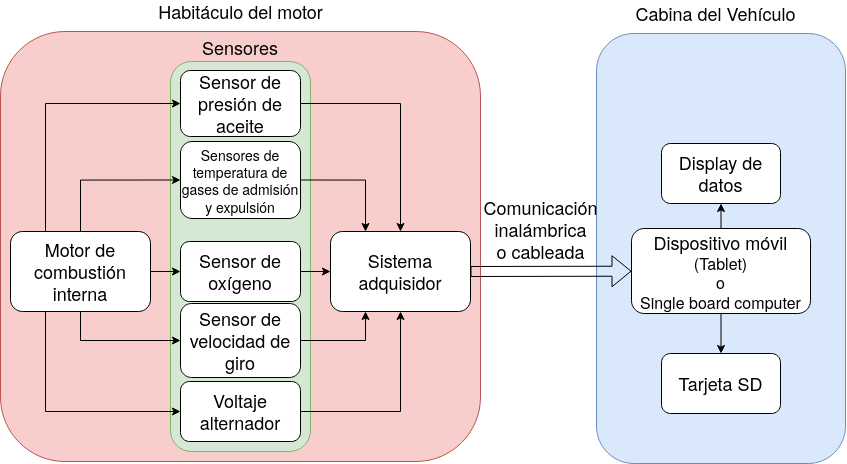
\includegraphics[width=.9\textwidth]{./Figuras/diagrama-proyecto.png}
\caption{Diagrama en bloques del sistema}
\label{fig:diagrama_de_bloques}
\end{figure}

\vspace{25px}

Lo que se quiere lograr con este sistema es que el usuario pueda ver en tiempo real en qué condiciones se encuentra funcionando el motor. Con esta información disponible se le otorga al usuario la capacidad de diagnosticar fallas antes de que le ocurran daños graves al motor. Se pretende ofrecer un gran aporte de valor a aquellas personas propietarias de vehículos antiguos que no tienen esta tecnología incorporada, dado que es muy costoso mantenerlos en funcionamiento óptimo, más que nada por la dificultad de conseguir repuestos. El sistema también tiene la posibilidad de aportar un gran valor en instituciones educativas técnicas que brinden enseñanza en la temática, brindando un contexto visual a fenómenos del funcionamiento de un motor que no podrían verse de otra forma.

Por esto es que se apunta a comercializar al sistema en forma de kit de sencilla instalación, apuntado a propietarios de automotores antiguos con intereses técnicos, mecánicos y también a instituciones educativas del rubro.

\section{Identificación y análisis de los interesados}
\label{sec:interesados}

\begin{table}[ht]
%\caption{Identificación de los interesados}
%\label{tab:interesados}
\begin{tabularx}{\linewidth}{@{}|l|X|X|l|@{}}
\hline
\rowcolor[HTML]{C0C0C0} 
Rol           & Nombre y Apellido & Organización 	& Puesto 	\\ \hline
%Auspiciante   & -                  						& -             	& -       	\\ \hline
Cliente       & \clientename      						&\empclientename	& -      	\\ \hline
%Impulsor      & -                 						& -            		& -       	\\ \hline
Responsable   & \authorname       						& LSE - FIUBA  		& Alumno 	\\ \hline
%Colaboradores & -                  						& -            		& -       	\\ \hline
Orientador    & \supname	      						& \pertesupname 	& Director \\ \hline
%Equipo        & -		         						& -            		& -      	\\ \hline
%Opositores    & -                  						& -            		& -        	\\ \hline
Usuario final & Propietarios de Vehículos antiguos, \newline  
				Mećanicos e Instituciones Educativas \newline  &            & \\ \hline
\end{tabularx}
\end{table}

\section{1. Propósito del proyecto}
\label{sec:proposito}

El propósito de este proyecto es el de desarrollar y construir un prototipo del sistema, instalarlo en una Volkswagen Tipo 2 modelo 1985 y analizar el funcionamiento de su motor en base a los datos visualizados.

\section{2. Alcance del proyecto}
\label{sec:alcance}

El alcance de este proyecto incluye:
\begin{itemize}
\item La elección de componentes electrónicos.
\item El diseño del circuito para amplificar las señales de los sensores.
\item El diseño del circuito impreso.
\item El desarrollo del firmware de la parte adquisidora.
\item El desarrollo del software de la interfaz gráfica de usuario.
\item La confección de un primer prototipo.
\item Los ensayos de verificación y validación con el prototipo.
\end{itemize}

El proyecto no incluye:
\begin{itemize}
\item La elección o desarrollo de un gabinete para la parte adquisidora.
\item El desarrollo de los componentes de montaje del sistema adquisidor.
\item El montaje del dispositivo para la interfaz gráfica en la cabina del vehículo.
\item La elección de sensores a utilizar.
\item Desarrollo del embalaje y documentación acompañante (e.g.: manual de usuario, prospecto).
\end{itemize}

\section{3. Supuestos del proyecto}
\label{sec:supuestos}

Para el desarrollo del presente proyecto se supone que:

\begin{itemize}
\item Los sensores ya fueron seleccionados, y que se cuenta con un sensor de oxígeno marca bosch y dos termocuplas para sensar la temperatura de los gases de admisión y escape, y también sensores para la temperatura y presión de aceite.
\item El resto de los materiales serán adquiridos por el Cliente.
\item Se cuenta con una placa EDU-CIAA sobre la cuál se desarrollará el firmware de la parte adquisidora.
\item Se cuenta con una tablet con pantalla táctil, puerto micro USB-OTG que corre sistema operativo Android.
\item Se supone que será fácil de conseguir las herramientas necesarias para el desarrollo y construcción del primer prototipo y su instalación en el vehículo. (e.g.: multímetro, osciloscopio, destornilladores, llaves, etc).
\end{itemize}

\section{4. Requerimientos}
\label{sec:requerimientos}

\begin{itemize}
\item Requerimientos generales del proyecto:
	\begin{itemize}
	\item \textbf{REQ-GEN-001:} Todo el código fuente del proyecto será almacenado bajo un sistema de control de versiones GIT.
	\item \textbf{REQ-GEN-002:} La documentación del código fuente del software embebido será llevada a cabo en los comentarios, siguiendo el formato de Doxygen.
	\item \textbf{REQ-GEN-003:} La documentación del software para la interfaz gráfica también será llevada a cabo en los comentarios. El formato será elegido por el responsable del proyecto.
	\end{itemize}
\item Requerimientos de la interfaz gráfica de usuario:
	\begin{itemize}
	\item \textbf{REQ-GUI-001:} La interfaz gráfica deberá poder mostrar figuras con la información de todos los sensores a la vez.
	\item \textbf{REQ-GUI-002:} El usuario tiene que poder elegir qué sensores ver al mismo tiempo y cuáles no desea ver.
	\item \textbf{REQ-GUI-003:} El usuario tiene que poder definir alarmas por valor máximo, para cada una de las variables.
	\item \textbf{REQ-GUI-004:} Las alarmas serán sonoras y visuales. El estilo de las alarmas será definido por el cliente durante el proceso de desarrollo de la interfaz gráfica.

	\end{itemize}
\item Requerimientos de la parte adquisidora:
	\begin{itemize}
	\item \textbf{REQ-ADQ-001:} El sistema tiene que adquirir la temperatura de los gases de admisión y escape, con un rango de temperatura entre 0"oC y 400"oC y una resolución menor igual a 0,5"oC. Con una tasa de muestreo mayor igual a 1hz.
	\item \textbf{REQ-ADQ-002:} El sistema tien que adquirir la temperatura del aceite del motor, con un rango de temperatura ente 0"oC y 400"oC y una resolución menor igual a 0,5"oC. Con una tasa de muestreo mayor igual a 1hz.
	\item \textbf{REQ-ADQ-003:} El sistema tiene que adquirir la velocidad de giro del motor, en un rango entre 0 y 20.000 revoluciones por minuto, con una resolución menor igual a 500 r.p.m. Con una tasa de muestreo mayor igual a 5hz.
	\item \textbf{REQ-ADQ-004:} El sistema tiene que adquirir la proporción de oxígeno en los gases de escape llamada lambda, con un rango de 0 a 2 y una resolución menor igual a 0,1 lambda.
	\item \textbf{REQ-ADQ-005:} El sistema tiene que adquirir la presión de aceite del motor, con un rango de 0 a 100 psi y con una resolución menor igual a 1 psi.
	\item \textbf{REQ-ADQ-006:} El sistema debe comenzar a transmitir a la interfaz gráfica la información obtenida de los sensores en un tiempo no mayor a 1 segundo transcurrido el proceso de adquisición.
	
	\end{itemize}
\item Requerimientos de la comunicación entre las partes del sistema:
	\begin{itemize}
	\item \textbf{REQ-COMM-001:} Se permitirá que se pierda hasta 1 de cada 100 paquetes transmitidos.	
	\end{itemize}
\end{itemize}

\section{Historias de usuarios (\textit{Product backlog})}
\label{sec:backlog}

\begin{itemize}
\item \textbf{HU-001:} Como cliente quiero poder visualizar en una pantalla la información de los sensores en tiempo real en un mismo gráfico lineal.
	\begin{itemize}
	\item Ponderación: La historia de usuario es clara, su complejidad es media y no es muy abarcativa, pero el desarrollador tiene poca experiencia programando interfaces gráficias. Se asignan 8 puntos de historia.
	\end{itemize}
\item \textbf{HU-002:} Como cliente quiero poder definir la escala del eje temporal del gráfico lineal, pudiendo elegir entre cinco valores distintos. (1 minuto, 10 minutos, 30 minutos, 60 minutos y 120 minutos).
	\begin{itemize}
	\item Ponderación: La historia de usuario es sencilla y no debería abarcar mucho trabajo. Pero como en esta etapa todavía no se conoce como se implementarán los gráficos se le asignan 2 puntos de historia.
	\end{itemize}
\item \textbf{HU-003:} Como cliente quiero poder elegir que sensores deben ser mostrados en pantalla y cuales no, para poder darle prioridad a la información que es más relevante en ese momento.
	\begin{itemize}
	\item Ponderación: Se le asignan a esta historia de usuario 2 puntos de historia. Las razones son las mismas que para HU-002.
	\end{itemize}
\item \textbf{HU-004:} Como cliente quiero poder definir niveles para cada sensor individualmente, y que suene una alarma cuando algún valor supere dicho nivel para ser notificado al instante de que algo no funciona adecuadamente.
	\begin{itemize}
	\item Ponderación: Esta tarea es de complejidad media porque involucra reproducción de archivos de audio. Además en esta etapa todavía no esta completamente definido como será el sonido de la alarma. Se le asignan 8 puntos de historia.
	\end{itemize}
\item \textbf{HU-005:} Como cliente quiero poder descargar toda la información recolectada en una tarjeta SD o pendrive, para poder analizarla en otro momento.
	\begin{itemize}
	\item Ponderación: Volcar la información que está almacenada en la memoria no volátil del hardware de la interfaz gráfica a una tarjeta SD o pendrive no es una tarea muy compleja, aunque aún falta definir el tamaño y formato de la información a descargar. Se asignan 5 puntos de historia.
	\end{itemize}
\item \textbf{HU-006:} Como cliente quiero que el sistema comience a funcionar cuando se le da contacto al vehículo con la llave de ignición.
	\begin{itemize}
	\item Ponderación: La historia de usuario es bastante clara. Pero es bastante compleja porque se deberá estudiar como funcionan los circuitos de ignición de un vehículo y diseñar un circuito que energice al sistema con el contacto de la llave. Se asignan 13 puntos de historia.
	\end{itemize}
\end{itemize}

\section{5. Entregables principales del proyecto}
\label{sec:entregables}

\begin{itemize}
\item Código fuente del firmware.
\item Código fuente del software de interfaz gráfica.
\item Documentación del firmware y software.
\item Esquemático del circuito.
\item Proyecto del circuito impreso.
\item Circuito impreso con componentes soldados en funcionamiento.
\item Memoria final.
\end{itemize}

\section{6. Desglose del trabajo en tareas}
\label{sec:wbs}

\begin{enumerate}
\item \textbf{Planificación.} (60 hs)
	\begin{enumerate}
	\item Plan de trabajo. (20 hs)
	\item Especificación de requerimientos de sistema. (20 hs)
	\item Definición de pruebas de verificación y validación. (20 hs)
	\end{enumerate}
\item \textbf{Diseño y construcción del hardware del equipo.} (65 hs)
	\begin{enumerate}
	\item Selección de componentes electrónicos. (10 hs)
	\item Diseño del esquemático del circuito. (20 hs)
	\item Diseño del circuito impreso. (20 hs)
	\item Diseño del esquema de interconexión entre las partes. (5 hs)
	\item Montaje del prototipo. (10 hs)
	\end{enumerate}
\item \textbf{Diseño de la interfaz gráfica.} (165 hs)
	\begin{enumerate}
	\item Diseño de la arquitectura de software. (30 hs)
	\item Maquetación de la interfaz gráfica. (30 hs)
	\item Desarrollo del software. (30 hs)
	\item Pruebas de verificación. (30 hs)
	\item Modificaciones del software. (15 hs)
	\item Segunda ronda de pruebas de verificación. (30hs).
	\end{enumerate}
\item \textbf{Diseño e implementación del firmware} (170 hs).
	\begin{enumerate}
	\item Diseño de la arquitectura de software. (20)
	\item Instalación y familiarización con el entorno de desarrollo. (15 hs)
	\item Diseño del módulo adquisidor de temperaturas. (10hs)
	\item Diseño del módulo adquisidor de presión de aceite. (10 hs)
	\item Diseño del módulo adquisidor de relación de oxígeno. (10 hs)
	\item Diseño del módulo de transmisión de datos. (30 hs)
	\item Pruebas de verificación. (30hs hs)
	\item Modificaciones del software. (15hs hs)
	\item Segunda ronda de pruebas de verificación. (30hs hs).
	\end{enumerate}
\item \textbf{Etapa de validación.} (50 hs)
	\begin{enumerate}
	\item Pruebas de validación con el prototipo montado sobre el vehículo. (30hs)
	\item Ajustes luego de las pruebas de validación. (20hs)
	\end{enumerate}
\item \textbf{Cierre del proyecto.} (90 hs)
	\begin{enumerate}
	\item Informes de avance del proyecto (20hs)
	\item Redacción de la memoría final del proyecto (40hs)
	\item Correcciones a la memoria final del proyecto (20hs)
	\item Presentación final del proyecto (10hs).
	\end{enumerate}
\end{enumerate}

Cantidad total de horas: (600 hs)


\section{7. Diagrama de Activity On Node}
\label{sec:AoN}

\begin{consigna}{red}
Armar el AoN a partir del WBS definido en la etapa anterior. 

%La figura \ref{fig:AoN} fue elaborada con el paquete latex tikz y pueden consultar la siguiente referencia \textit{online}:

%\url{https://www.overleaf.com/learn/latex/LaTeX_Graphics_using_TikZ:_A_Tutorial_for_Beginners_(Part_3)\%E2\%80\%94Creating_Flowcharts}

\end{consigna}

\begin{figure}[htpb]
\centering 
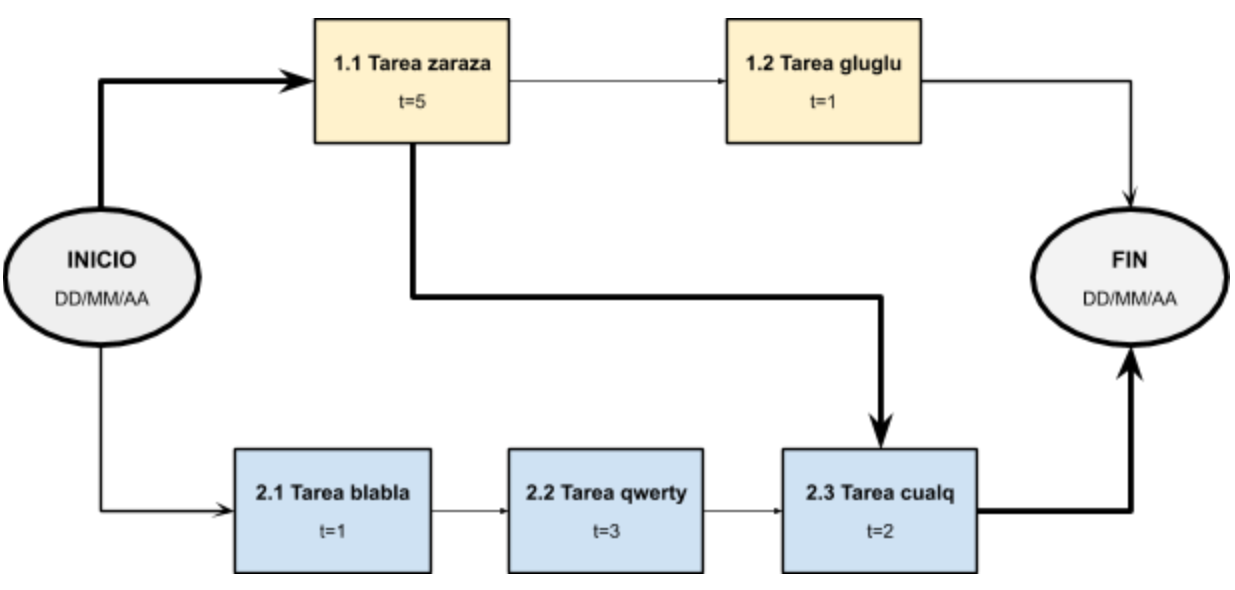
\includegraphics[width=.8\textwidth]{./Figuras/AoN.png}
\caption{Diagrama en \textit{Activity on Node}}
\label{fig:AoN}
\end{figure}

Indicar claramente en qué unidades están expresados los tiempos.
De ser necesario indicar los caminos semicríticos y analizar sus tiempos mediante un cuadro.
Es recomendable usar colores y un cuadro indicativo describiendo qué representa cada color, como se muestra en el siguiente ejemplo:



\section{8. Diagrama de Gantt}
\label{sec:gantt}

\begin{consigna}{red}
Utilizar el software Gantter for Google Drive o alguno similar para dibujar el diagrama de Gantt.

Existen muchos programas y recursos \textit{online} para hacer diagramas de gantt, entre las cuales destacamos:

\begin{itemize}
\item Planner
\item GanttProject
\item Trello + \textit{plugins}. En el siguiente link hay un tutorial oficial: \\ \url{https://blog.trello.com/es/diagrama-de-gantt-de-un-proyecto}
\item Creately, herramienta online colaborativa. \\\url{https://creately.com/diagram/example/ieb3p3ml/LaTeX}
\item Se puede hacer en latex con el paquete \textit{pgfgantt}\\ \url{http://ctan.dcc.uchile.cl/graphics/pgf/contrib/pgfgantt/pgfgantt.pdf}
\end{itemize}

Pegar acá una captura de pantalla del diagrama de Gantt, cuidando que la letra sea suficientemente grande como para ser legible. 
Si el diagrama queda demasiado ancho, se puede pegar primero la ``tabla'' del Gantt y luego pegar la parte del diagrama de barras del diagrama de Gantt.

Configurar el software para que en la parte de la tabla muestre los códigos del EDT (WBS).\\
Configurar el software para que al lado de cada barra muestre el nombre de cada tarea.\\
Revisar que la fecha de finalización coincida con lo indicado en el Acta Constitutiva.

En la figura \ref{fig:gantt}, se muestra un ejemplo de diagrama de gantt realizado con el paquete de \textit{pgfgantt}. En la plantilla pueden ver el código que lo genera y usarlo de base para construir el propio.

\begin{figure}[htbp]
\begin{center}
\begin{ganttchart}{1}{12}
  \gantttitle{2020}{12} \\
  \gantttitlelist{1,...,12}{1} \\
  \ganttgroup{Group 1}{1}{7} \\
  \ganttbar{Task 1}{1}{2} \\
  \ganttlinkedbar{Task 2}{3}{7} \ganttnewline
  \ganttmilestone{Milestone o hito}{7} \ganttnewline
  \ganttbar{Final Task}{8}{12}
  \ganttlink{elem2}{elem3}
  \ganttlink{elem3}{elem4}
\end{ganttchart}
\end{center}
\caption{Diagrama de gantt de ejemplo}
\label{fig:gantt}
\end{figure}

\end{consigna}

\section{9. Matriz de uso de recursos de materiales}
\label{sec:recursos}


\begin{table}
\label{tab:recursos}
\centering
\begin{tabularx}{\linewidth}{@{}|c|X|X|X|X|c|@{}}
\hline
\cellcolor[HTML]{C0C0C0} & \cellcolor[HTML]{C0C0C0} & \multicolumn{4}{c|}{\cellcolor[HTML]{C0C0C0}Recursos requeridos (horas)} \\ \cline{3-6} 
\multirow{-2}{*}{\cellcolor[HTML]{C0C0C0}\begin{tabular}[c]{@{}c@{}}Código\\ WBS\end{tabular}} & \multirow{-2}{*}{\cellcolor[HTML]{C0C0C0}\begin{tabular}[c]{@{}c@{}}Nombre \\ tarea\end{tabular}} & Material 1 & Material 2 & Material 3 & Material 4 \\ \hline
 &  &  &  &  &  \\ \hline
 &  &  &  &  &  \\ \hline
 &  &  &  &  &  \\ \hline
 &  &  &  &  &  \\ \hline
 &  &  &  &  &  \\ \hline
 &  &  &  &  &  \\ \hline
 &  &  &  &  &  \\ \hline
 &  &  &  &  &  \\ \hline 
 &  &  &  &  &  \\ \hline
 &  &  &  &  &  \\ \hline
 &  &  &  &  &  \\ \hline
 &  &  &  &  &  \\ \hline
 &  &  &  &  &  \\ \hline
 &  &  &  &  &  \\ \hline
 &  &  &  &  &  \\ \hline
 &  &  &  &  &  \\ \hline
 &  &  &  &  &  \\ \hline
 &  &  &  &  &  \\ \hline
 &  &  &  &  &  \\ \hline
 &  &  &  &  &  \\ \hline
 &  &  &  &  &  \\ \hline
 &  &  &  &  &  \\ \hline
 &  &  &  &  &  \\ \hline
 &  &  &  &  &  \\ \hline 
 &  &  &  &  &  \\ \hline
 &  &  &  &  &  \\ \hline
 &  &  &  &  &  \\ \hline
 &  &  &  &  &  \\ \hline

\end{tabularx}%
\end{table}


\section{10. Presupuesto detallado del proyecto}
\label{sec:presupuesto}

\begin{consigna}{red}
Si el proyecto es complejo entonces separarlo en partes:
\begin{itemize}
\item Un total global, indicando el subtotal acumulado por cada una de las áreas.
\item El desglose detallado del subtotal de cada una de las áreas.
\end{itemize}

IMPORTANTE: No olvidarse de considerar los COSTOS INDIRECTOS.

\end{consigna}

\begin{table}[htpb]
\centering
\begin{tabularx}{\linewidth}{@{}|X|c|r|r|@{}}
\hline
\rowcolor[HTML]{C0C0C0} 
\multicolumn{4}{|c|}{\cellcolor[HTML]{C0C0C0}COSTOS DIRECTOS} \\ \hline
\rowcolor[HTML]{C0C0C0} 
Descripción &
  \multicolumn{1}{c|}{\cellcolor[HTML]{C0C0C0}Cantidad} &
  \multicolumn{1}{c|}{\cellcolor[HTML]{C0C0C0}Valor unitario} &
  \multicolumn{1}{c|}{\cellcolor[HTML]{C0C0C0}Valor total} \\ \hline
 &
  \multicolumn{1}{c|}{} &
  \multicolumn{1}{c|}{} &
  \multicolumn{1}{c|}{} \\ \hline
 &
  \multicolumn{1}{c|}{} &
  \multicolumn{1}{c|}{} &
  \multicolumn{1}{c|}{} \\ \hline
\multicolumn{1}{|l|}{} &
   &
   &
   \\ \hline
\multicolumn{1}{|l|}{} &
   &
   &
   \\ \hline
\multicolumn{3}{|c|}{SUBTOTAL} &
  \multicolumn{1}{c|}{} \\ \hline
\rowcolor[HTML]{C0C0C0} 
\multicolumn{4}{|c|}{\cellcolor[HTML]{C0C0C0}COSTOS INDIRECTOS} \\ \hline
\rowcolor[HTML]{C0C0C0} 
Descripción &
  \multicolumn{1}{c|}{\cellcolor[HTML]{C0C0C0}Cantidad} &
  \multicolumn{1}{c|}{\cellcolor[HTML]{C0C0C0}Valor unitario} &
  \multicolumn{1}{c|}{\cellcolor[HTML]{C0C0C0}Valor total} \\ \hline
\multicolumn{1}{|l|}{} &
   &
   &
   \\ \hline
\multicolumn{1}{|l|}{} &
   &
   &
   \\ \hline
\multicolumn{1}{|l|}{} &
   &
   &
   \\ \hline
\multicolumn{3}{|c|}{SUBTOTAL} &
  \multicolumn{1}{c|}{} \\ \hline
\rowcolor[HTML]{C0C0C0}
\multicolumn{3}{|c|}{TOTAL} &
   \\ \hline
\end{tabularx}%
\end{table}


\section{11. Matriz de asignación de responsabilidades}
\label{sec:responsabilidades}
\begin{consigna}{red}
Establecer la matriz de asignación de responsabilidades y el manejo de la autoridad completando la siguiente tabla:

\begin{table}[htpb]
\centering
\resizebox{\textwidth}{!}{%
\begin{tabular}{|c|c|c|c|c|c|}
\hline
\rowcolor[HTML]{C0C0C0} 
\cellcolor[HTML]{C0C0C0} &
  \cellcolor[HTML]{C0C0C0} &
  \multicolumn{4}{c|}{\cellcolor[HTML]{C0C0C0}Listar todos los nombres y roles del proyecto} \\ \cline{3-6} 
\rowcolor[HTML]{C0C0C0} 
\cellcolor[HTML]{C0C0C0} &
  \cellcolor[HTML]{C0C0C0} &
  Responsable &
  Orientador &
  Equipo &
  Cliente \\ \cline{3-6} 
\rowcolor[HTML]{C0C0C0} 
\multirow{-3}{*}{\cellcolor[HTML]{C0C0C0}\begin{tabular}[c]{@{}c@{}}Código\\ WBS\end{tabular}} &
  \multirow{-3}{*}{\cellcolor[HTML]{C0C0C0}Nombre de la tarea} &
  \authorname &
  \supname &
  Nombre de alguien &
  \clientename \\ \hline
 &  &  &  &  &  \\ \hline
 &  &  &  &  &  \\ \hline
 &  &  &  &  &  \\ \hline
\end{tabular}%
}
\end{table}

{\footnotesize
Referencias:
\begin{itemize}
	\item P = Responsabilidad Primaria
	\item S = Responsabilidad Secundaria
	\item A = Aprobación
	\item I = Informado
	\item C = Consultado
\end{itemize}
} %footnotesize

Una de las columnas debe ser para el Director, ya que se supone que participará en el proyecto.
A su vez se debe cuidar que no queden muchas tareas seguidas sin ``A'' o ``I''.

Importante: es redundante poner ``I/A'' o ``I/C'', porque para aprobarlo o responder consultas primero la persona debe ser informada.

\end{consigna}

\section{12. Gestión de riesgos}
\label{sec:riesgos}

\begin{consigna}{red}
a) Identificación de los riesgos (al menos cinco) y estimación de sus consecuencias:
 
Riesgo 1: detallar el riesgo (riesgo es algo que si ocurre altera los planes previstos)
\begin{itemize}
\item Severidad (S): mientras más severo, más alto es el número (usar números del 1 al 10).\\
Justificar el motivo por el cual se asigna determinado número de severidad (S).
\item Probabilidad de ocurrencia (O): mientras más probable, más alto es el número (usar del 1 al 10).\\
Justificar el motivo por el cual se asigna determinado número de (O). 
\end{itemize}   

Riesgo 2:
\begin{itemize}
\item Severidad (S): 
\item Ocurrencia (O):
\end{itemize}

Riesgo 3:
\begin{itemize}
\item Severidad (S): 
\item Ocurrencia (O):
\end{itemize}


b) Tabla de gestión de riesgos:      (El RPN se calcula como RPN=SxO)

\begin{table}[htpb]
\centering
\begin{tabularx}{\linewidth}{@{}|X|c|c|c|c|c|c|@{}}
\hline
\rowcolor[HTML]{C0C0C0} 
Riesgo & S & O & RPN & S* & O* & RPN* \\ \hline
       &   &   &     &    &    &      \\ \hline
       &   &   &     &    &    &      \\ \hline
       &   &   &     &    &    &      \\ \hline
       &   &   &     &    &    &      \\ \hline
       &   &   &     &    &    &      \\ \hline
\end{tabularx}%
\end{table}

Criterio adoptado: 
Se tomarán medidas de mitigación en los riesgos cuyos números de RPN sean mayores a...

Nota: los valores marcados con (*) en la tabla corresponden luego de haber aplicado la mitigación.

c) Plan de mitigación de los riesgos que originalmente excedían el RPN máximo establecido:
 
Riesgo 1: plan de mitigación (si por el RPN fuera necesario elaborar un plan de mitigación).
  Nueva asignación de S y O, con su respectiva justificación:
  - Severidad (S): mientras más severo, más alto es el número (usar números del 1 al 10).
          Justificar el motivo por el cual se asigna determinado número de severidad (S).
  - Probabilidad de ocurrencia (O): mientras más probable, más alto es el número (usar del 1 al 10).
          Justificar el motivo por el cual se asigna determinado número de (O).

Riesgo 2: plan de mitigación (si por el RPN fuera necesario elaborar un plan de mitigación).
 
Riesgo 3: plan de mitigación (si por el RPN fuera necesario elaborar un plan de mitigación).

\end{consigna}


\section{13. Gestión de la calidad}
\label{sec:calidad}

\begin{consigna}{red}
Para cada uno de los requerimientos del proyecto indique:
\begin{itemize} 
\item Req \#1: copiar acá el requerimiento.

Verificación y validación:

\begin{itemize}
\item Verificación para confirmar si se cumplió con lo requerido antes de mostrar el sistema al cliente. Detallar 
\item Validación con el cliente para confirmar que está de acuerdo en que se cumplió con lo requerido. Detallar  
\end{itemize}

\end{itemize}

Tener en cuenta que en este contexto se pueden mencionar simulaciones, cálculos, revisión de hojas de datos, consulta con expertos, mediciones, etc.

\end{consigna}

\section{14. Comunicación del proyecto}
\label{sec:comunicaciones}

El plan de comunicación del proyecto es el siguiente:

\begin{table}[htpb]
\centering
\begin{tabularx}{\linewidth}{@{}|X|C{2.4cm}|C{3cm}|C{1.8cm}|C{2cm}|C{2.1cm}|@{}}
\hline
\rowcolor[HTML]{C0C0C0} 
\multicolumn{6}{|c|}{\cellcolor[HTML]{C0C0C0}PLAN DE COMUNICACIÓN DEL PROYECTO}           \\ \hline
\rowcolor[HTML]{C0C0C0} 
¿Qué comunicar? & Audiencia & Propósito & Frecuencia & Método de comunicac. & Responsable \\ \hline
                &           &           &            &                      &             \\ \hline
                &           &           &            &                      &             \\ \hline
                &           &           &            &                      &             \\ \hline
                &           &           &            &                      &             \\ \hline
                &           &           &            &                      &             \\ \hline
\end{tabularx}
\end{table}

\section{15. Gestión de compras}
\label{sec:compras}

\begin{consigna}{red}
En caso de tener que comprar elementos o contratar servicios:
a) Explique con qué criterios elegiría a un proveedor.
b) Redacte el Statement of Work correspondiente.
\end{consigna}

\section{16. Seguimiento y control}
\label{sec:seguimiento}

\begin{consigna}{red}
Para cada tarea del proyecto establecer la frecuencia y los indicadores con los se seguirá su avance y quién será el responsable de hacer dicho seguimiento y a quién debe comunicarse la situación (en concordancia con el Plan de Comunicación del proyecto).

El indicador de avance tiene que ser algo medible, mejor incluso si se puede medir en \% de avance. Por ejemplo,se pueden indicar en esta columna cosas como ``cantidad de conexiones ruteadeas'' o ``cantidad de funciones implementadas'', pero no algo genérico y ambiguo como ``\%'', porque el lector no sabe porcentaje de qué cosa.

\end{consigna}

\begin{longtable}{|m{1cm}|m{3.5cm}|m{2.2cm}|m{2cm}|m{3cm}|m{1.5cm}|}
\hline
\rowcolor[HTML]{C0C0C0} 
\multicolumn{6}{|c|}{\cellcolor[HTML]{C0C0C0}SEGUIMIENTO DE AVANCE}                                                                       \\ \hline
\rowcolor[HTML]{C0C0C0} 
Tarea del WBS 			& Indicador de avance & Frecuencia de reporte & Resp. de seguimiento & Persona a ser informada & Método de comunic. \\ \hline
\endfirsthead

\hline
\rowcolor[HTML]{C0C0C0} 
\multicolumn{6}{c}{\cellcolor[HTML]{C0C0C0}SEGUIMIENTO DE AVANCE}                                                                       \\ \hline
\rowcolor[HTML]{C0C0C0} 
Tarea del WBS 			& Indicador de avance & Frecuencia de reporte & Resp. de seguimiento & Persona a ser informada & Método de comunic. \\ \hline
\endhead

\multicolumn{6}{c}{Continúa}
\endfoot

\endlastfoot

1.1	& Fecha de inicio  & Única vez al comienzo & \authorname & \clientename, \supname & email \\ \hline
2.1	& Avance de las subtareas  & Mensual mientras dure la tarea & \authorname & \clientename, \supname & email \\ \hline

\end{longtable}

\begin{table}[!htpb]
\centering
%\begin{tabularx}{\linewidth}{@{}|X|X|X|X|X|X|@{}}
\begin{tabularx}{\linewidth}{@{}|X|C{2.5cm}|C{3cm}|C{2cm}|C{2cm}|C{2.5cm}|@{}}
\hline
\rowcolor[HTML]{C0C0C0} 
\multicolumn{6}{|c|}{\cellcolor[HTML]{C0C0C0}SEGUIMIENTO DE AVANCE}                                                                       \\ \hline
\rowcolor[HTML]{C0C0C0} 
Tarea del WBS & Indicador de avance & Frecuencia de reporte & Resp. de seguimiento & Persona a ser informada & Método de comunic. \\ \hline
 &  &  &  &  &  \\ \hline
 &  &  &  &  &  \\ \hline
 &  &  &  &  &  \\ \hline
 &  &  &  &  &  \\ \hline
 &  &  &  &  &  \\ \hline
\end{tabularx}%
%}
\end{table}

\section{17. Procesos de cierre}    
\label{sec:cierre}

\begin{consigna}{red}
Establecer las pautas de trabajo para realizar una reunión final de evaluación del proyecto, tal que contemple las siguientes actividades:

\begin{itemize}
\item Pautas de trabajo que se seguirán para analizar si se respetó el Plan de Proyecto original:
 - Indicar quién se ocupará de hacer esto y cuál será el procedimiento a aplicar. 
\item Identificación de las técnicas y procedimientos útiles e inútiles que se utilizaron, y los problemas que surgieron y cómo se solucionaron:
 - Indicar quién se ocupará de hacer esto y cuál será el procedimiento para dejar registro.
\item Indicar quién organizará el acto de agradecimiento a todos los interesados, y en especial al equipo de trabajo y colaboradores:
  - Indicar esto y quién financiará los gastos correspondientes.
\end{itemize}

\end{consigna}


\end{document}
